\documentclass[12pt]{article}
\usepackage[utf8]{inputenc}
\usepackage[T1]{fontenc}
\usepackage[polish]{babel}
\usepackage{geometry}
\usepackage{tabularx}
\usepackage[table,xcdraw,dvipsnames]{xcolor}
\usepackage{color}
\usepackage{subfig}
\usepackage{sidecap}
\usepackage{wrapfig}
\usepackage{float}
\usepackage{enumerate}
\usepackage{graphicx}
\usepackage{multirow}
\usepackage{hyperref}
\usepackage{titlesec}
\usepackage{amsmath}
\usepackage{anyfontsize}
\usepackage{indentfirst}
\usepackage{listings}
\usepackage{multicol}
\usepackage{pgfplots}
\usepackage{fancyhdr}

\newgeometry{tmargin=1.8cm,bmargin=1.8cm,lmargin =1.8cm,rmargin=1.8cm}
\begin{document}

\begin{titlepage}
\begin{figure}
    \centering
    
\includegraphics[width=18cm]{logo-PWr.png}
    \label{fig:pwr}
\end{figure}
    \begin{center}
        \LARGE \textbf{ Wydział Elektroniki, Fotoniki i Mikrosystemów }\\ 
        \vspace{70pt}
        \Huge \textit{ Sterowanie Procesami Ciągłymi}  \\
    \end{center}
    \vspace{30pt}
    \hrule
    \vspace{1pt}
    \hrule
    \begin{center}
        {\fontsize{30}{50}\selectfont Sprawozdanie nr 1\\ }
        \vspace{10pt}
        {\fontsize{25}{25}\selectfont Charakterystyki czasowe  }
    \end{center}
    \hrule
    \vspace{1pt}
    \hrule
    \begin{flushright}
        \vspace{50pt}

        \textit{\Large Prowadzący:}\\
        \Large dr hab. inż. Grzegorz Mzyk\\
        \vspace{10pt}
        \textit{\Large Wykonała:}\\
        \Large Zuzanna Mejer, 259382 \\
        \vspace{10pt}
        \textit{\Large Termin zajęć:}\\
        \Large czwartek TP, 9:15\\
        \vspace{10pt}
    
    \end{flushright}
    \vspace{60pt}
    \begin{center}
        \large Wrocław, \today r.
    \end{center}
\end{titlepage}
    
    
\tableofcontents
\newpage

\section{Cel ćwiczenia}
Celem ćwiczenia jest zapoznanie się z charakterystykami czasowymi systemów. Ćwiczenie można podzielić na dwie części - badanie systemu z czasem ciągłym oraz dyskretnym. Zapoznano się z zależnością charakterystyki skokowej od położenia biegunów transmitancji układów zarówno z czasem ciągłym jak i dyskretnym. Podjęta została także próba identyfikacji systemów z czasem ciągłym i dyskretnym na podstawie charakterystyk skokowych.


\section{Badanie systemów z czasem ciągłym}

Rozpatrywany jest system ciągły o transmitancji w postaci:
\begin{equation}
    K(s) = \frac{1}{s^2+as+b},
\end{equation}
którą można przedstawić również jako:
\begin{equation}
    K(s) = \frac{1}{(s+b_1)(s+b_2)},
\end{equation}
gdzie $b_1$ oraz $b_2$ to bieguny. W zależności od ich położenia badano odpowiedź skokową układu.

\subsection{Położenie biegunów a odpowiedź skokowa układu}

\subsubsection{Bieguny rzeczywiste, ujemne}
Przyjmując wartości biegunów:
\begin{equation*}
    \left\{{{b_1 = -3}\atop {b_2 = -2}}\right.
\end{equation*}

Transmitancja systemu to:
\begin{equation}
    K(s) = \frac{1}{(s-(-3))(s-(-2))} = \frac{1}{(s+3)(s+2)} = \frac{1}{s^2+5s+6}
\end{equation}

Wygenerowano odpowiedź skokową systemu:

\begin{figure}[H]
    \centering
    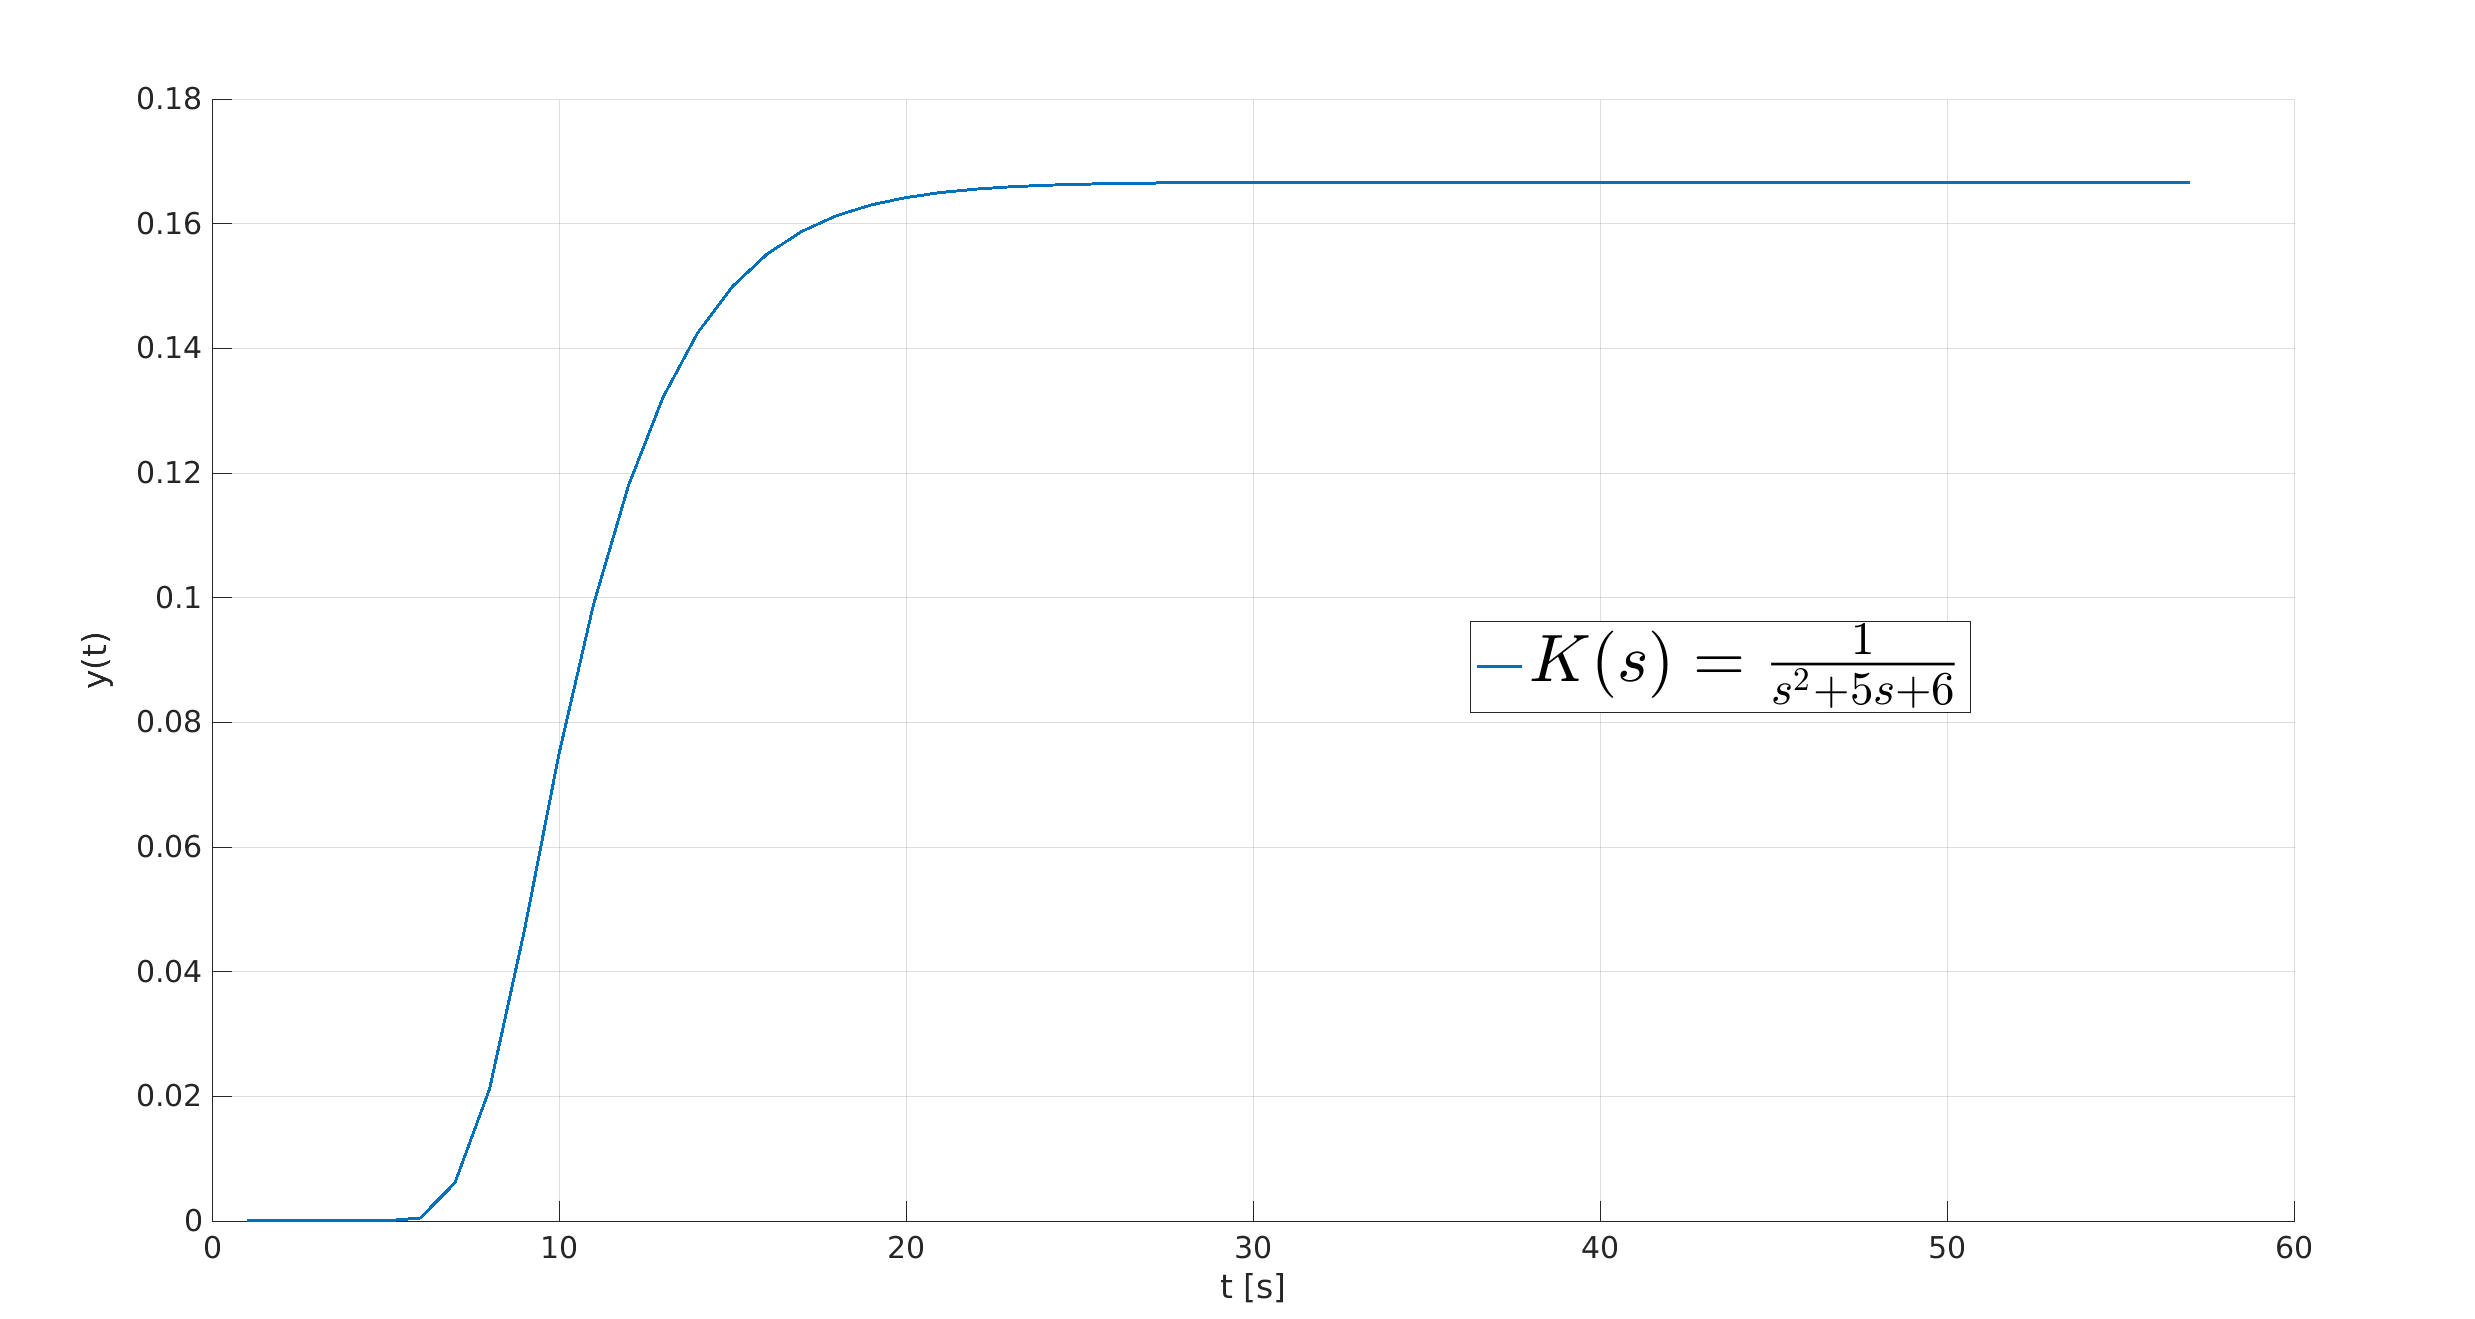
\includegraphics[width=18cm]{rzeczywiste_ujemne.png}
    \caption{Odpowiedź skokowa układu o transmitancji, której obydwa bieguny są rzeczywiste i ujemne}
\end{figure}



\colorbox{WildStrawberry}{tutaj z matlaba}

Układ jest stabilny (stabilizuje się na wartości \colorbox{WildStrawberry}{jakiej}) oraz nie ma oscylacji.


\subsubsection{Bieguny rzeczywiste o przeciwnych znakach}

Przyjmując wartości biegunów:
\begin{equation*}
    \left\{{{b_1 = -1}\atop {b_2 = 2}}\right.
\end{equation*}

Transmitancja systemu to:
\begin{equation}
    K(s) = \frac{1}{(s-(-1))(s-(2))} = \frac{1}{(s+1)(s-2)} = \frac{1}{s^2-s-2}
\end{equation}

Wygenerowano odpowiedź skokową systemu:
\colorbox{WildStrawberry}{tutaj z matlaba}

\begin{figure}[H]
    \centering
    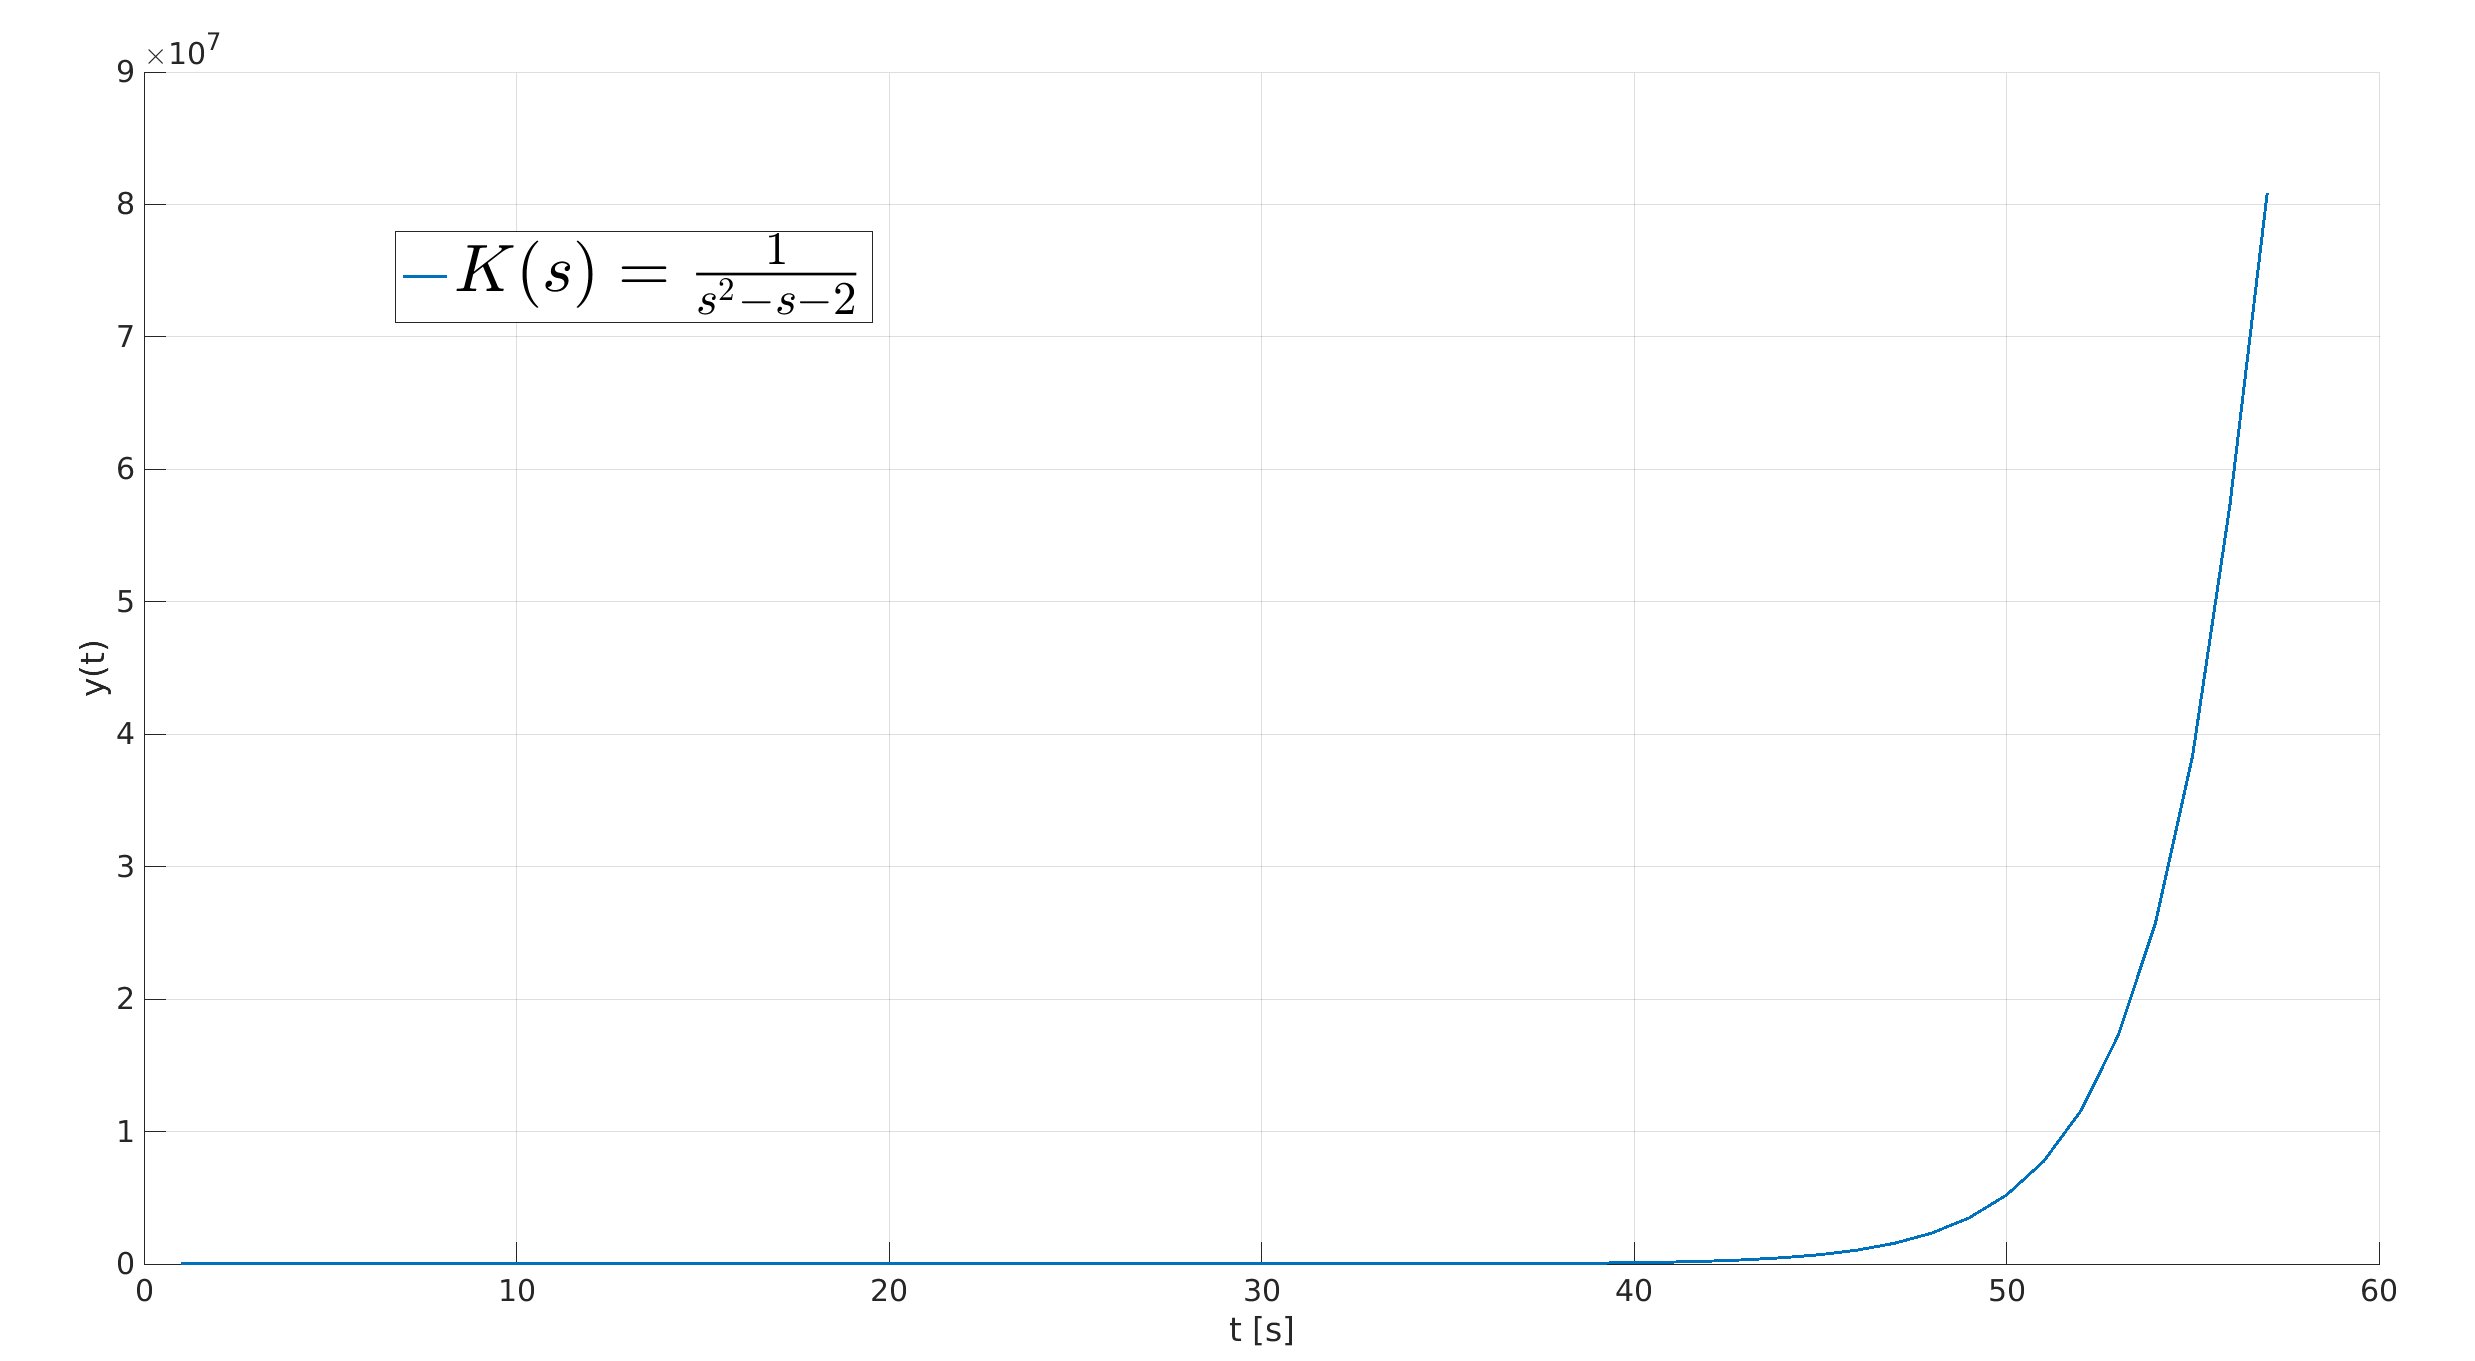
\includegraphics[width=18cm]{rzeczywiste_przeciwne_znaki.png}
    \caption{Odpowiedź skokowa układu o transmitancji, której bieguny mają przeciwne znaki}
\end{figure}

Układ nie jest stabilny oraz nie ma oscylacji.


\subsubsection{Bieguny zespolone z ujemną częścią rzeczywistą}

Przyjmując wartości biegunów:
\begin{equation*}
    \left\{{{b_1 = \frac{-0,1 + j \sqrt{3,99}}{2}}\atop {b_2 = \frac{-0,1 - j \sqrt{3,99}}{2}}}\right.
\end{equation*}

Transmitancja systemu to:
\begin{equation}
    K(s) = \frac{1}{(s-(\frac{-0,1 - j \sqrt{3,99}}{2}))(s-(\frac{-0,1 - j \sqrt{3,99}}{2}))} = \frac{1}{s^2+0,1s+1}
\end{equation}

Wygenerowano odpowiedź skokową systemu:
\colorbox{WildStrawberry}{tutaj z matlaba}

\begin{figure}[H]
    \centering
    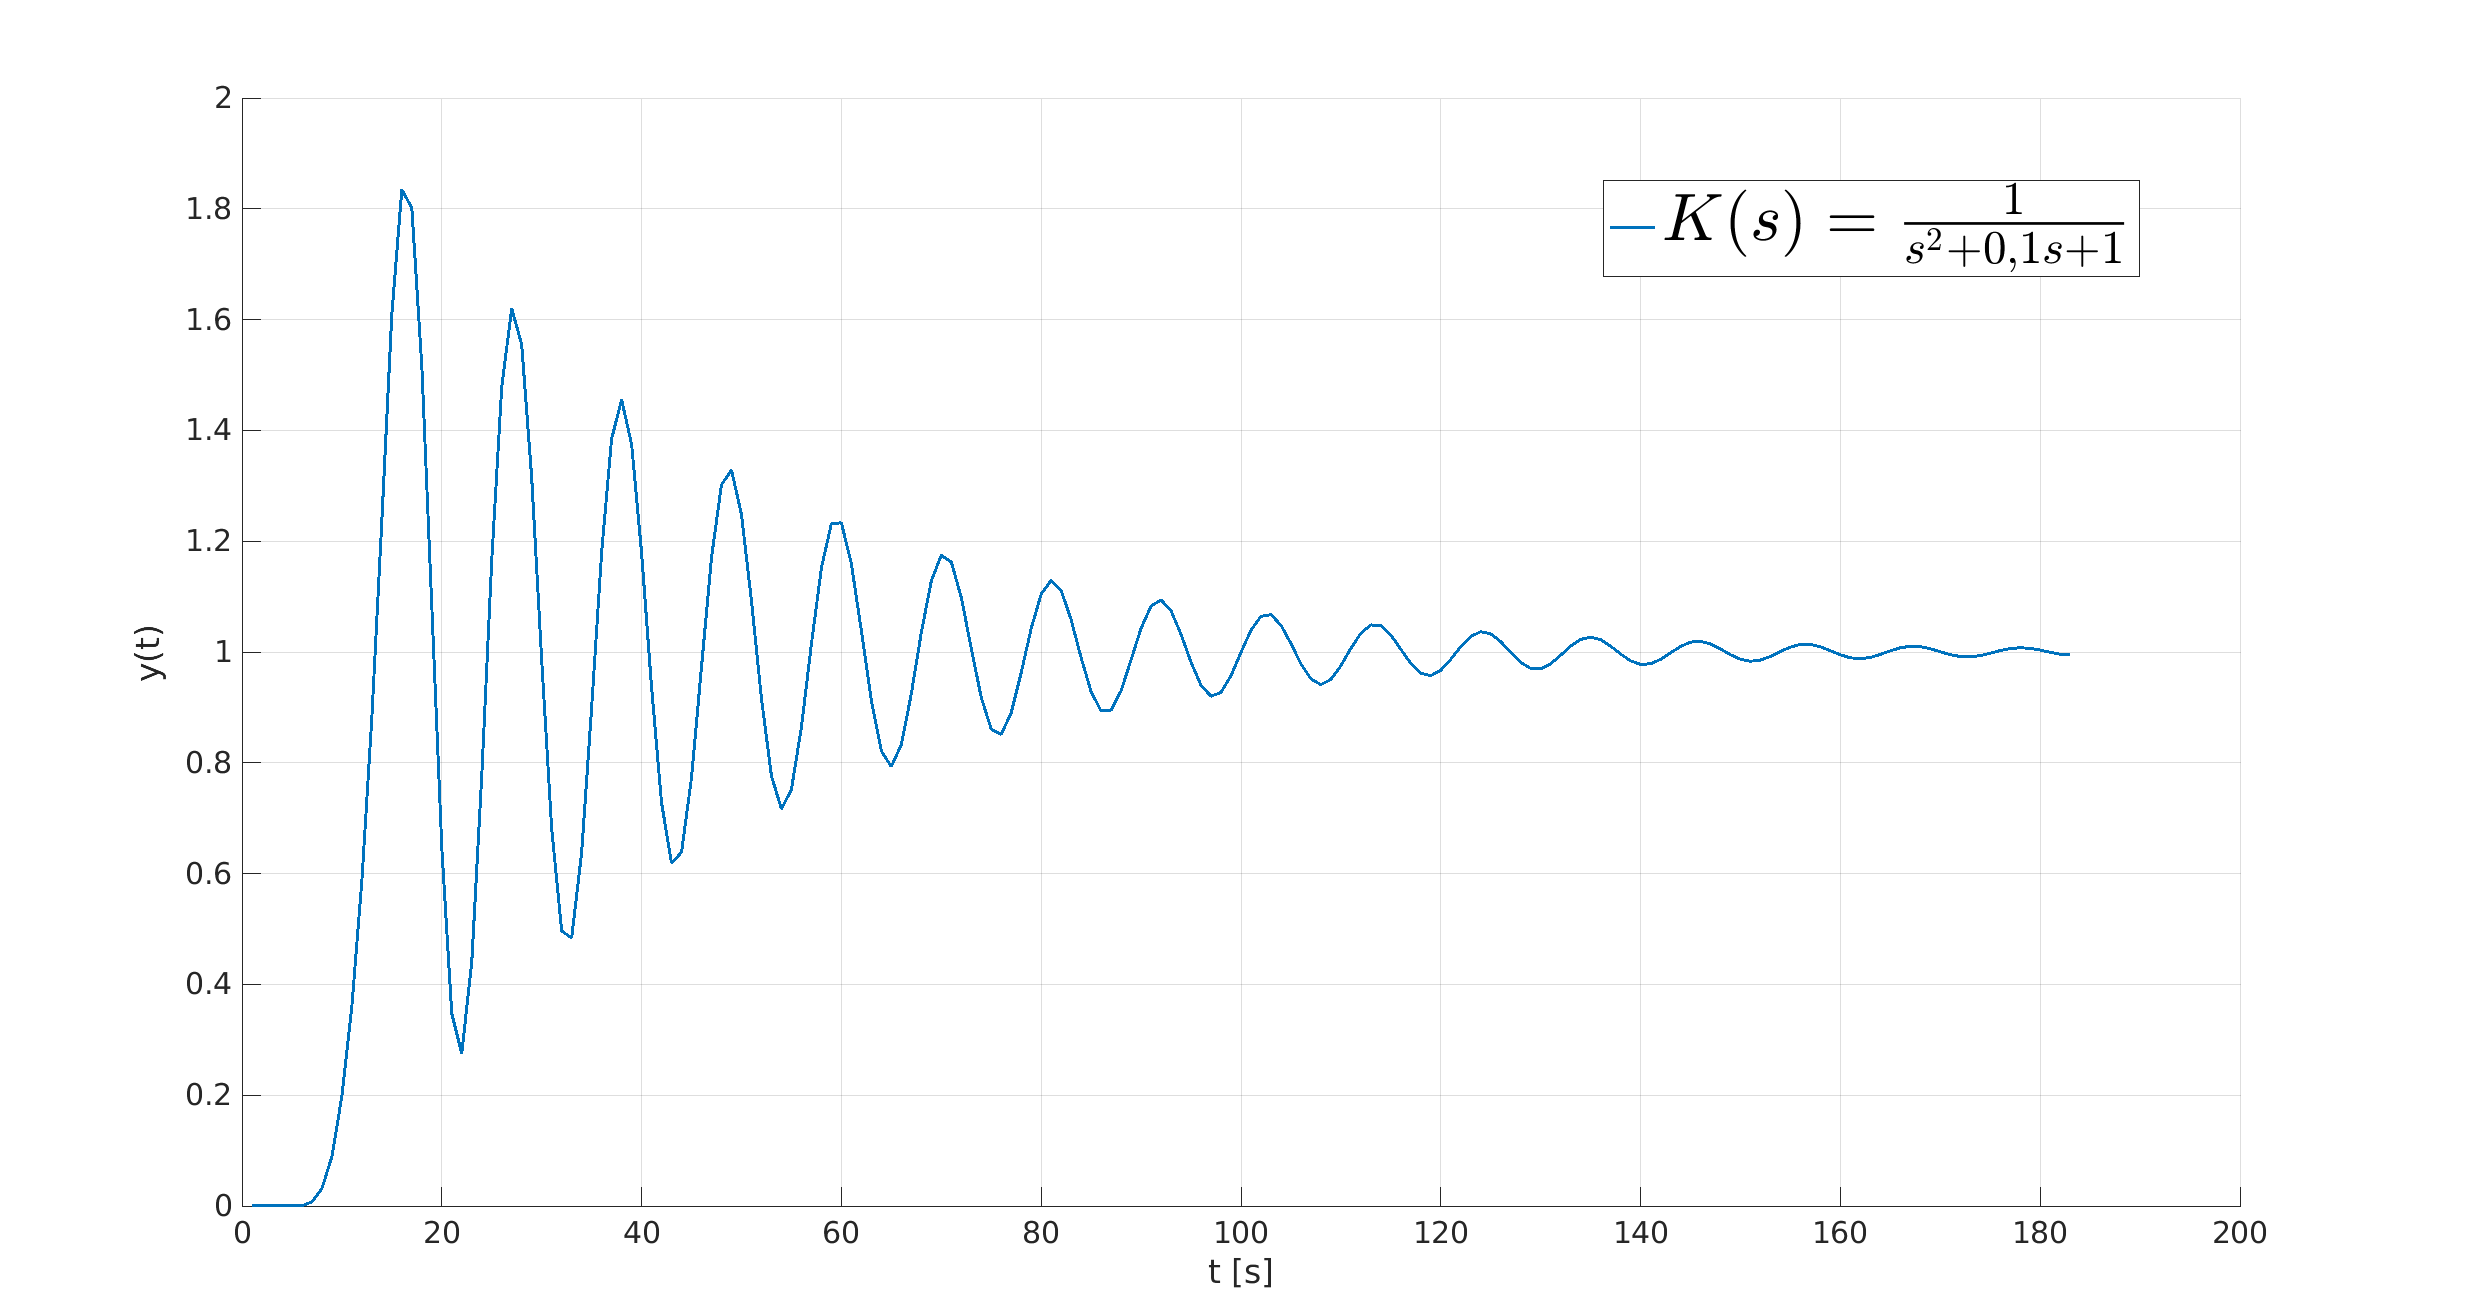
\includegraphics[width=18cm]{zespolone_ujemne.png}
    \caption{Odpowiedź skokowa układu o transmitancji, której bieguny są zespolone a ujemną częścią rzeczywistą}
\end{figure}

Układ jest stabilny (stabilizuje się na wartości \colorbox{WildStrawberry}{jakiej}) oraz ma oscylacje.

\subsubsection{Bieguny zespolone z dodatnią częścią rzeczywistą}

Przyjmując wartości biegunów:
\begin{equation*}
    \left\{{{b_1 = \frac{0,1 + j \sqrt{3,99}}{2}}\atop {b_2 = \frac{0,1 - j \sqrt{3,99}}{2}}}\right.
\end{equation*}

Transmitancja systemu to:
\begin{equation}
    K(s) = \frac{1}{(s-(\frac{0,1 - j \sqrt{3,99}}{2}))(s-(\frac{0,1 - j \sqrt{3,99}}{2}))} = \frac{1}{s^2-0,1s+1}
\end{equation}

Wygenerowano odpowiedź skokową systemu:
\colorbox{WildStrawberry}{tutaj z matlaba}

\begin{figure}[H]
    \centering
    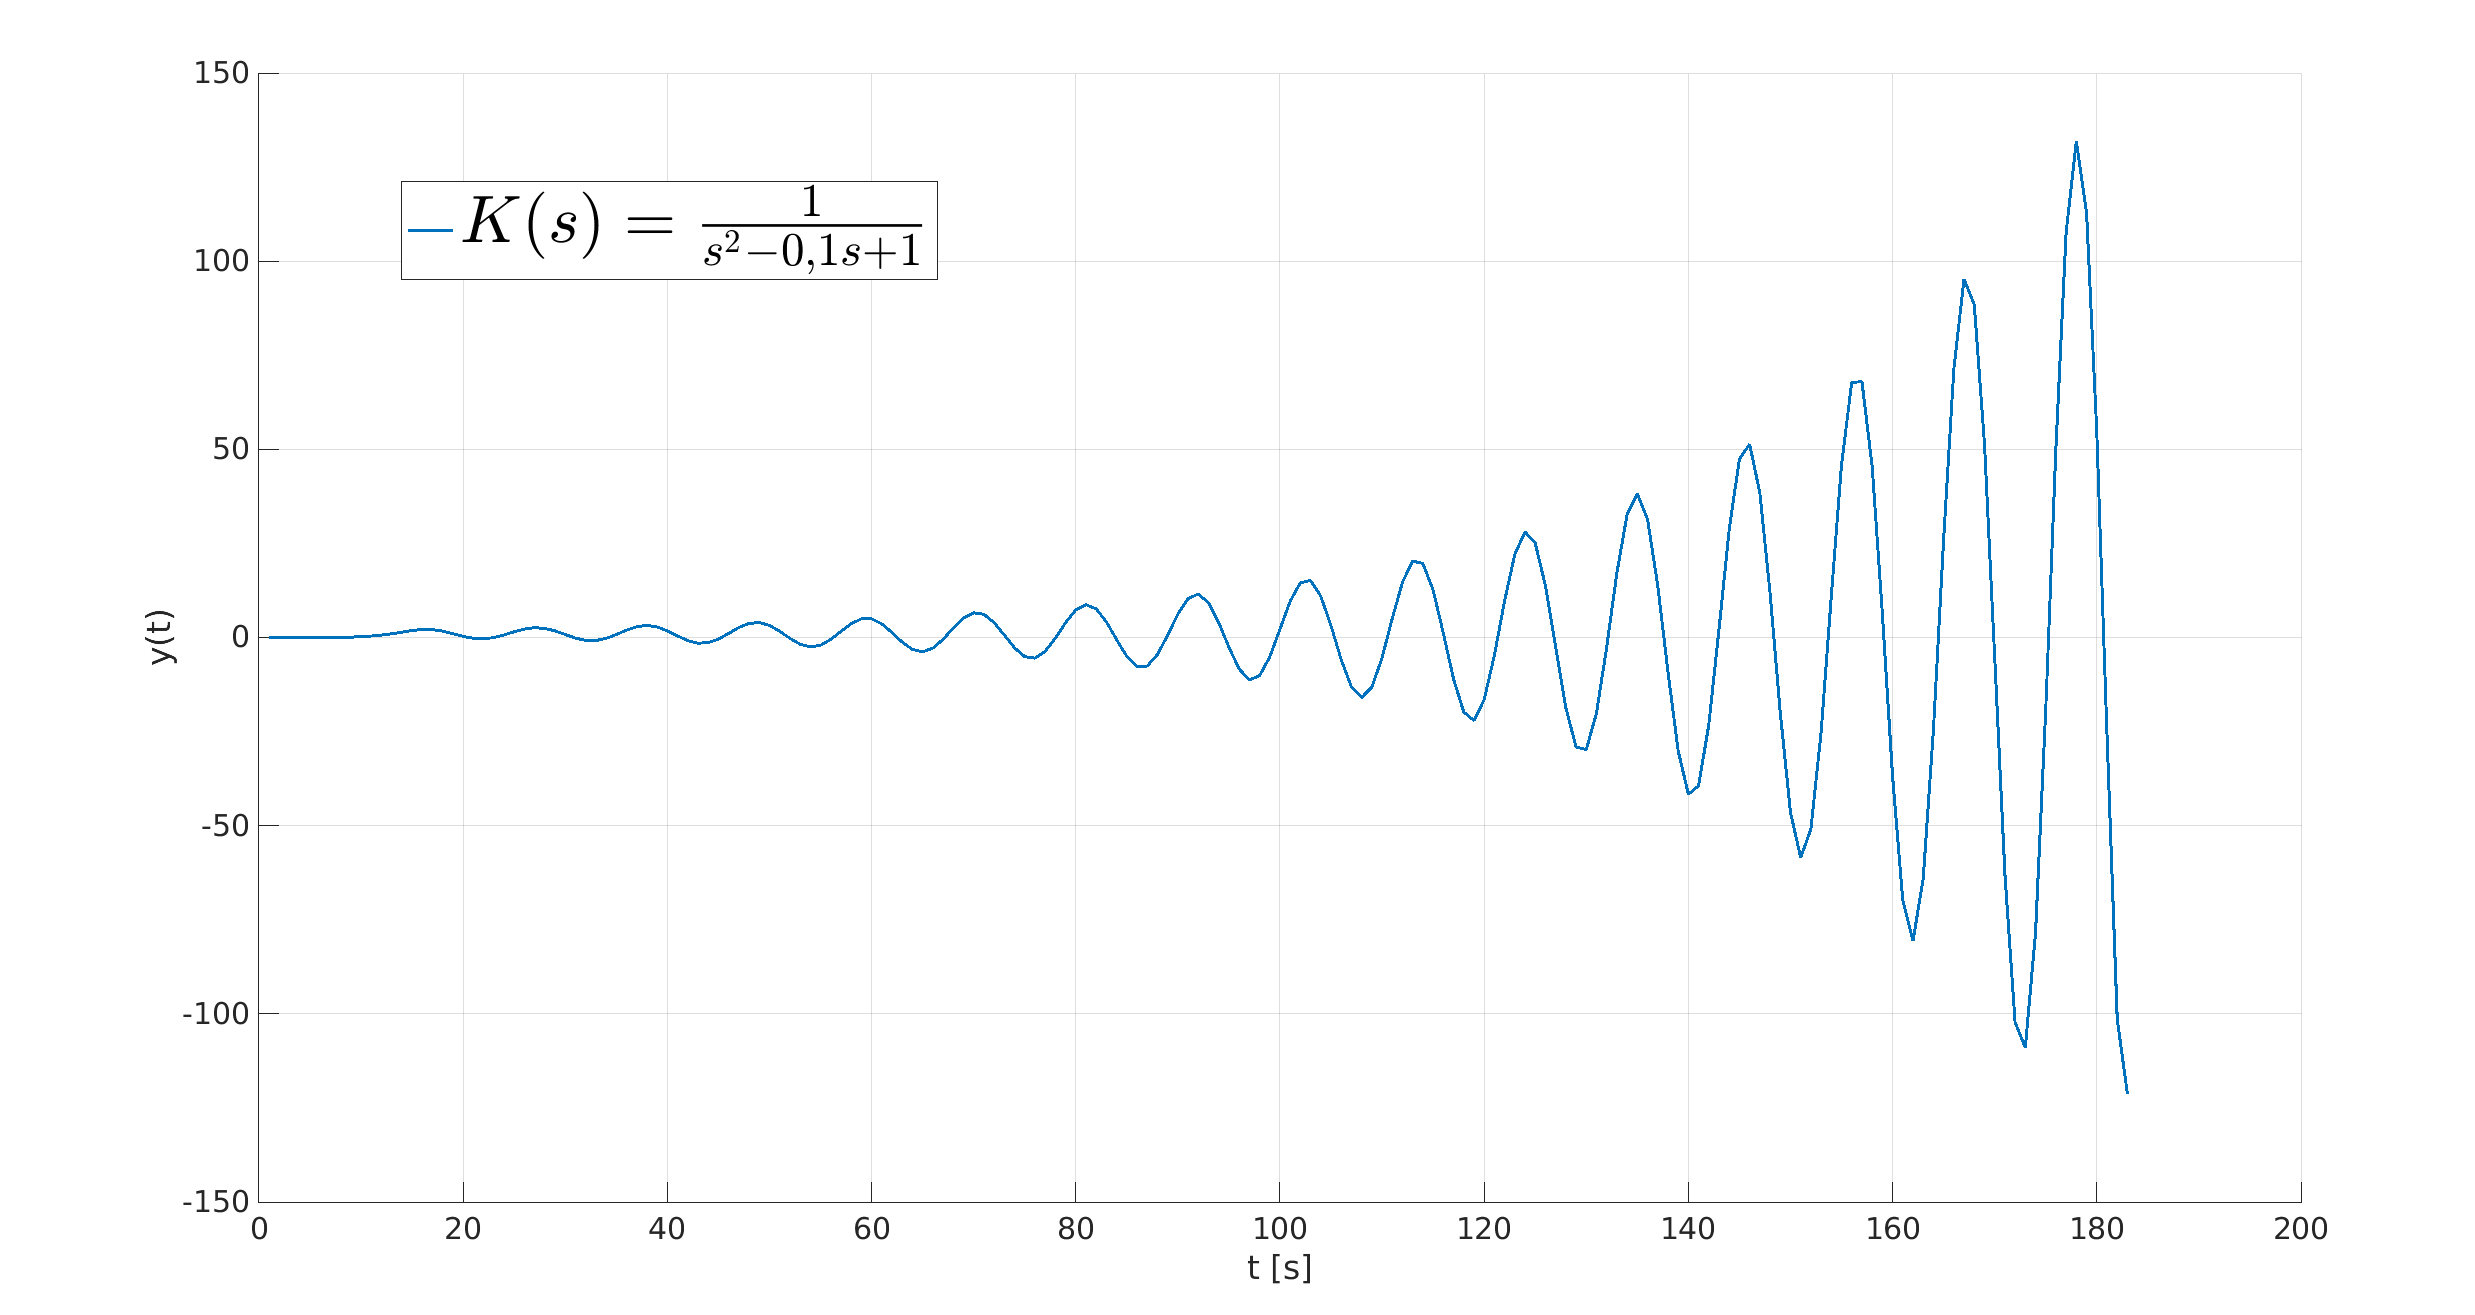
\includegraphics[width=18cm]{zespolone_dodatnia.png}
    \caption{Odpowiedź skokowa układu o transmitancji, której bieguny są zespolone z dodatnią częścią rzeczywistą}
\end{figure}

Układ nie jest stabilny oraz ma oscylacje.


\subsection{Identyfikacja systemów z czasem ciągłym na podstawie odpowiedzi skokowej}
\subsubsection{Bieguny rzeczywiste, ujemne}

Odpowiedź skokowa wygląda następująco:



\subsubsection{Bieguny rzeczywiste o przeciwnych znakach}
\subsubsection{Bieguny zespolone z ujemną częścią rzeczywistą}
\subsubsection{Bieguny zespolone z dodatnią częścią rzeczywistą}

\subsubsection{Porównanie wyników identyfikacji z rzeczywistymi wartościami}

\section{Badanie systemów z czasem dyskretnym}

\section{Podsumowanie i wnioski}

\section{Bibliografia}
\begin{enumerate}
    \item
%    \item https://www.dbc.wroc.pl/Content/16126/PDF/czempik_praktyczne.pdf
%   \item https://eia.pg.edu.pl/documents/1113028/0/WwT14_KSS_2014_2015_Obiekty_sterowania_i_ich_identyfikacja.pdf
\end{enumerate}

\end{document}